\chapter{Quantenmechanik}

\section{Grundlagen}

\begin{enumerate}[i)]
	\item \textbf{Wellenfunktion} $ \Psi(\vec{r}) $ $ \qquad $ mit $ \vec{r} $ der \textbf{Ortsdarstellung}
	\begin{equation*}
	P = \int_{V} \left|\Psi ( \vec{r})\right|^2 \dd \vec{r} \quad \tx{Wahrscheinlichkeit} \qquad \quad \int_{V} \left|\Psi(\vec{r})\right|^2 \dd \vec{r} = 1 \quad \tx{Normierungsbedingung}
	\end{equation*}
	\item \textbf{Operatoren} $ \hat{\mathcal{O}} $
	\begin{equation*}
	\hat{\mathcal{O}} \Psi(\vec{r}) = \Psi'(\vec{r})
	\end{equation*}
	Korrespondenzprinzip
	\begin{align*}
	\vec{r} &= \hat{\vec{r}} \qquad \hat{\vec{r}} \Psi(\vec{r}) = \Psi'(\vec{r}) = \vec{r} \Psi(\vec{r}) \qquad \quad ; \quad \, \rmbox{\hat{x} \Psi(x) = x \Psi(x) = \Psi'(x)} \\
	\vec{p} &= \hat{\vec{p}} \qquad \hat{\vec{p}} \Psi(\vec{r}) = \Psi'(\vec{r}) = - i \hbar \vabla \Psi(\vec{r}) \quad ; \quad \rmbox{\hat{p}_{x} \Psi(x) = - i \hbar \prd{}{x} \Psi(x) = \Psi'(x) }
	\end{align*}
	$ \hat{\ham} = $ Hamiltonian oder Hamilton-Operator. $ \hat{\ham} = \hat{\ham}(\hat{\vec{r}} , \hat{\vec{p}}) $
	\begin{equation*}
	\hat{\ham} = \frac{\hat{p^2}}{2m} + V(\vec{r}) = - \frac{\hbar^2}{2m} \vabla^2 + V(\vec{r})
	\end{equation*}
	\item \textbf{Zeitabhängige Schrödinger Gleichung}
	\begin{equation*}
	\rmbox{i\hbar \prt{}{t} \Psi(\vec{r}, t) = \hat{\ham}  \Psi(\vec{r}, t)}
	\end{equation*}
	Die klassische Energie sieht so aus:
	\begin{equation*}
	E = \frac{p^2}{2m} + V(\vec{r})
	\end{equation*}
	In der QM dann folgendermaßen:
	\begin{equation*}
	\hat{\ham} = \frac{\hat{p}^2}{2m} + V(\vec{r})
	\end{equation*}
	Die \textbf{Zeitunabhängige Schrödinger Gleichung} sieht wie folgt aus:
	\begin{equation*}
	\rmbox{\hat{\ham} \Psi(\vec{r}) = E \Psi(\vec{r})}
	\end{equation*}
	Diese Gleichung ist eine Eingenwertgleichung. Der Hamilton Operator liefert also den Energie-Eingenwert $ E $ und die Eigenzustände $ \Psi(\vec{r}) $.
	
	\subsection*{Stationäre Zustände}
	
	Jeder messbaren Physikalische Größe ist ein Operator $ \hat{\mathcal{O}} $ zugeordnet. Bei einer physikalischen Messung wird der \textbf{Erwartungswert} gemessen: $ \langle \hat{\mathcal{O}} \rangle = \langle \Psi | \hat{\mathcal{O}} | \Psi \rangle $.
	\begin{equation*}
	\langle \hat{\mathcal{O}} \rangle = \langle \Psi(\vec{r}) | \hat{\mathcal{O}} | \Psi(\vec{r}) \rangle = \int \Psi^*(\vec{r}) \ \ub{ \hat{O} \ \ \Psi(\vec{r}) }_{\Psi'(\vec{r})} \dd \vec{r}
	\end{equation*}
	\begin{equation*}
	\langle \hat{\mathcal{O}}(t) \rangle = \langle \Psi(\vec{r},t) | \hat{\mathcal{O}} | \Psi(\vec{r},t) \rangle = \int \Psi^*(\vec{r},t) \hat{\mathcal{O}} \Psi(\vec{r},t) \dd \vec{r}
	\end{equation*}
	Diese Gleichung können wir wie folgt umformen:
	\begin{equation*}
	\Psi(\vec{r},t) = \Psi(\vec{r},t = 0) \ub{e^{- \nicefrac{i E t}{\hbar}}}_{\tx{Phasenfaktor}}
	\end{equation*}
	\begin{align*}
	\langle \hat{\mathcal{O}} \rangle &= \int \Psi^*(\vec{r}, t = 0) \cancel{e^{\nicefrac{i E t}{\hbar}}} \hat{O} \Psi(\vec{r}, t = 0) \cancel{e^{- \nicefrac{i E t}{\hbar}}} \dd \vec{r} \\
	&= \int \Psi^*(\vec{r}, t = 0) \hat{\mathcal{O}} \Psi(\vec{r} , t = 0) \dd \vec{r} \overset{*}{=} \langle \hat{O}(t = 0) \rangle
	\end{align*}
	$ *: $ wenn $ \hat{\mathcal{O}} $ nicht Zeitabhängig ist.\\[5pt]
	\textbf{Stationäre Zustände}
	\begin{equation*}
	i \hbar \prt{}{t} \Psi(\vec{r}, t) = \hat{\ham} \Psi(\vec{r}, t) \qquad \tx{mit} \qquad \Psi(\vec{r},t) e^{- \frac{i E t}{\hbar}} \Psi(\vec{r} ,t = 0)
	\end{equation*}
	\begin{equation*}
	\frac{\partial \Psi}{\Psi} = - i \frac{\hat{\ham}}{\hbar} \partial t
	\end{equation*}
	Lösung der DGL mittels Variablen-Trennung
	\begin{equation*}
	\ln\left[\frac{\Psi(\vec{r},t)}{\Psi(\vec{r}, t = 0)}\right] = - \frac{i \hat{\ham} t}{\hbar} \quad \Rightarrow \quad \Psi(\vec{r}, t) = e^{- \frac{i \hat{\ham} t}{\hbar}} \Psi(\vec{r}, t = 0)
	\end{equation*}
	\begin{equation*}
	\hat{\ham} \Psi(\vec{r} , t = 0) = E \Psi(\vec{r}, t = 0)
	\end{equation*}
	Taylor Entwicklung:
	\begin{equation*}
	e^{x} = e^{- \frac{i \hat{\ham} t}{\hbar}} = a \left(\hat{\ham}\right)^0 + b \left(\hat{\ham}\right)^1 + c \left(\hat{\ham}\right)^2 + \dots
	\end{equation*}
	\begin{align*}
	e^{- \frac{i \hat{\ham} t}{\hbar}} \Psi(\vec{r}, t = 0)&= a \Psi(\vec{r}, t = 0) + b \hat{\ham} \Psi(\vec{r}, t = 0) + c \hat{\ham} \cdot \hat{\ham} \Psi(\vec{r}, t = 0) + \dots \\
	&= a \Psi(\vec{r}, t = 0) + b E \Psi(\vec{r}, t = 0) + c E^2 \Psi(\vec{r}, t = 0) + \dots \\
	&= (a + bE + c E^2 + \dots) \cdot \Psi(\vec{r}, t = 0) \\
	&= e^{- \frac{i E t}{\hbar}} \Psi(\vec{r}, t = 0)
	\end{align*}
	\lcom{Wir können einen Operator in der $ e $-Funktion schreiben, da diese mit der Taylorentwicklung als Reihe entwickelt werden kann.}
	\item \textbf{Spin} (Elektronen)
	\begin{enumerate}[$ \Rightarrow $]
		\item Wasserstoffatom (Stern-Gerlach)
		\item Helium (Pauli Prinzip)
	\end{enumerate}
	\newpage
	\item \textbf{Quantensysteme}
	\begin{itemize}
		\item Freies Teilchen, Potentialstufe (Tunneln)
		\item Harmonischer Oszillator $ \Rightarrow $ Molekülphysik
		\item Coulomb Potential $ \Rightarrow $ Wasserstoffatom
	\end{itemize}
	\begin{figure}[ht]
		\centering
		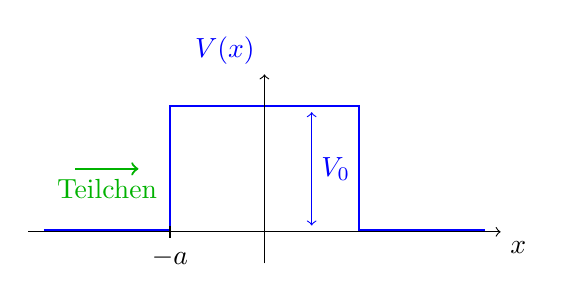
\begin{tikzpicture}[scale=0.8]
		\draw[thick,blue] (-3.5,.025) -| (-1.5,2) -- (1.5,2) |- (3.5,.025);
		\draw[thick,black!30!green,->] (-3,1) -- node[below] {Teilchen} ++(1,0);
		\draw[->] (-3.75,0) -- (3.75,0) node[anchor=north west] {$ x $};
		\draw[->] (0,-0.5) -- (0,2.5) node[anchor=south east] {\color{blue}$ V(x) $};
		\draw (-1.5,.1) -- ++(0,-.2) node[below] {$ -a $};
%		\draw (1.5,.1) -- ++(0,-.2) node[below] {$ +a $};
%		\node[draw=black,circle, minimum size=.8cm,red] at (-2.5,-1) {I};
%		\node[draw=black,circle, minimum size=.8cm,red] at (0,-1) {II};
%		\node[draw=black,circle, minimum size=.8cm,red] at (2.5,-1) {III};
		\draw[<->,blue] (.75,.1) -- node[right] {$ V_0 $} ++(0,1.8); 
		\end{tikzpicture}
		\label{Potentialbarriere}
		\caption{Darstellung einer Potentialbarriere. Beispiel für den Tunneleffekt eines hindurchfliegenden Teilchens, das eigentlich weniger Energie hat als klassisch nötig wäre um die Barriere zu überwinden. Dieses Bild wurde mit dem \LaTeX Paket Tikz erstellt.}
	\end{figure}
	\FloatBarrier
	\item \textbf{Kommutatoren}
	\begin{align*}
	\hat{x}&: \vec{p} = \vec{p}_x \qquad \qquad \left[\hat{x}, \hat{p}\right] = \hat{x} \hat{p} - \hat{p} \hat{x} \\
	\hat{A}; \hat{B}&: \qquad \qquad \qquad \ \left[\hat{A}, \hat{B}\right] = \hat{A} \hat{B} - \hat{B} \hat{A}
	\end{align*}
	Wellenfunktion $ \Psi(x) \qquad \qquad \left[\hat{x}, \hat{p}\right] \Psi(x) = \Psi'(x) $
	\begin{equation*}
	\left[\hat{x}, \hat{p}\right] = \hat{x} \hat{p} - \hat{p} \hat{x} = x \left(- i \hbar \prd{}{x}\right) - \left(- i \hbar \prd{}{x}\right) x
	\end{equation*}
	\begin{align*}
	\left[\hat{x}, \hat{p}\right] \Psi(x) &= \left\{ x \left(- i \hbar \prd{}{x}\right) - \left(- i \hbar \prd{}{x}\right) x \right\} \Psi(x) \\
	&= x \left(- i \hbar \prd{}{x} \Psi(x) \right) - \left(- i \hbar \prd{}{x}\right) x \Psi(x) \\
	&= - i \hbar x \prd{\Psi}{x} + i \hbar \prd{}{x} ( x \Psi(x)) \\
	&= \cancel{ - i \hbar x \prd{\Psi}{x}} \cancel{+ i \hbar x \prd{\Psi}{x}} + i \hbar \Psi(x) \ub{\prd{x}{x}}_{=1} \\
	&= i \hbar \Psi(x) = \Psi'(x)
	\end{align*}
	\begin{equation*}
	\rmbox{\left[\hat{x}, \hat{p}\right] = i \hbar} \quad \Rightarrow \quad \tx{die zwei Operatoren vertauschen nicht !!!}
	\end{equation*}
	
	\subsection*{Eigenschaft Kommutator}
	
	$ \hat{A} $; $ \hat{B} $
	\begin{equation*}
	\Delta A \cdot \Delta B \ge \frac{1}{2} \left| \left\langle \left[\hat{A}, \hat{B}\right] \right\rangle \right|
	\end{equation*}
	$ \left[\hat{A}, \hat{B}\right] $ Operator $ \Rightarrow $
	\begin{align*}
	\left\langle \left[\hat{A}, \hat{B}\right] \right\rangle &= \left\langle \hat{A} \hat{B} - \hat{B} \hat{A} \right\rangle \\
	&= \left\langle \Psi | \hat{A} \hat{B} - \hat{B} \hat{A} | \Psi \right\rangle \\
	&= \int \Psi^* \left(\hat{A} \hat{B} - \hat{B} \hat{A}\right) \Psi \dd \vec{r}
	\end{align*}
	$ \Delta A $, $ \Delta B $ Standardabweichung
	\begin{equation*}
	\sigma_x = P(x) \quad \sigma_x = \left[ \int (x - \mu)^2 P(x) \dd x \right]^{1/2}  \qquad \mu = \int x P(x) \dd x
	\end{equation*}
	
	% T Gaußglocke
	
	\begin{figure}
		\centering
		\begin{tikzpicture}
			\draw[->] (0,-0.2) -- (0,2.5) node[anchor=south east] {$ P(x) $};
			\draw[->] (-0.2,0) -- (7,0) node[anchor=north west] {$ x $};
			\draw[domain=0:7, samples=80, thick] plot (\x, {2*exp(-(\x - 3.5)^(2)*0.6});
			\coordinate (o) at (3.5,1);
			\coordinate (d) at (1.1,0);
			\draw[ultra thick, <->, blue, arrows = {Stealth}-{Stealth}] ($ (o) + (d) $) -- ($ (o) - (d) $);
		\end{tikzpicture}
		\label{Gausverteilung}
		\caption{Die Wahrscheinlichkeitsverteilung einer Gaußkurve. Der Pfeil soll die Standartabweichung darstellen. Dieses Bild wurde mit dem \LaTeX Paket Tikz erstellt.}
	\end{figure}
	
	$ \hat{A} = \hat{x} $, $ \hat{B} = \hat{p} $. $ \left[\hat{x}, \hat{p}\right] = i \hbar $
	\begin{equation*}
	\Delta A \cdot \Delta B \ge \frac{1}{2} \left| \left\langle \left[\hat{A}, \hat{B}\right] \right\rangle \right|
	\end{equation*}
	\begin{equation*}
	\Delta x \cdot \Delta p \ge \frac{1}{2} \left| i \hbar \right| = \frac{\hbar}{2}
	\end{equation*}	
\end{enumerate}

\subsection*{Morgen:}

Operatoren die vertauschen: Drehimpulsoperator $ \vec{l} $ mit den Komponenten $ l_x, l_y, l_z $ und $ l^2 $. Es gilt $ \left[l^2, l_z\right] = 0 $
\begin{equation*}
\Delta l^2 \cdot \Delta l_z \ge 0
\end{equation*}
Man kann also Zustände finden, bei denen $ \Delta l^2 = 0 $; $ \Delta l_z = 0 $ sind. Diese Zustände können im Prinzip existieren und verletzen die Unschärferelation nicht! Diese Zustände sind dann gleichzeitig Eigenzustände von $ l^2 $ und $ l_z $.

\subsubsection*{Exkurs: Varianz und Standardabweichung in der Quantenmechanik}

Wellenfunktion $ \Psi(x) $ mit Wahrscheinlichkeit $ P(x) = |\Psi(x)|^2 $
\begin{align*}
\mu &= \int x P(x) \dd x = \int x | \Psi(x) | ^2 \dd x \\
\sigma   &= \int x^2 P(x) \dd x = \int x^2 | \Psi(x) | ^2 \dd x
\end{align*}
Die Varianz ist definiert als:
\begin{align*}
\sigma^2 = \int (x - \mu)^2 P(x) \dd x &= \int (x^2 + \mu^2 - 2 \mu x) P(x) \dd x \\
&= \int x^2 P(x) \dd x + \mu^2 \int P(x) \dd x - 2 \mu \int x P(x) \dd x\\
&= \int x^2 P(x) \dd x + \mu^2 - 2 \mu \mu = \int x^2 P(x) \dd x - \mu^2 \\
&= \langle x ^2 \rangle - \langle x \rangle ^2
\end{align*}

% 26.04.19

\subsection*{Programm Heute}

\begin{itemize}
	\item Drehimpulsoperator
	\item Kugelflächenfunktionen (Wasserstoffatom)
	\item Vektormodell (klassische Darstellung)\\
	\lcom{Macht es leichter z.B. die Wechselwirkung zwischen Drehimpulsoperator und Magnetfeld zu verstehen. Dieses klassische Modell macht voraussagen über die QM.}
	\item Experimente (Spektrum des Wasserstoffatoms)
	\item Schrödinger Gleichung des Wasserstoffatoms
\end{itemize}

\section{Drehimpulsoperator}


\begin{minipage}{.5\linewidth}
	\begin{equation*}
	\vec{l} = \vec{r} \times \vec{p} = \vec{r} \times m \vec{v}
	\end{equation*}
	\begin{align*}
	\vec{r} & \Rightarrow \hat{\vec{r}} = \vec{r} \\
	\vec{p} & \Rightarrow \hat{ \vec{p}} = - i \hbar \vabla \\
	\vec{l} & \Rightarrow \hat{\vec{l}} = \vec{r} \times (- i \hbar \vabla) = - i \hbar \vec{r} \times \vabla
	\end{align*}
\end{minipage}%
\begin{minipage}{.5\linewidth}
	\flushright
	%t1:
	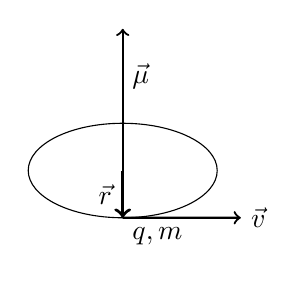
\begin{tikzpicture}[scale=.6]
		\draw[thick, ->] (0,0) -- (0,3);
		\draw (0,0) ellipse(2cm and 1cm);
		\coordinate (a) at (0,-1);
		\node[right] at (0,2) {$\vec{\mu}$};
		\node[anchor=north west] at (a) {$q,m$};
		\draw[very thick,->] (0,0) -- node[left] {$ \vec{r} $} (a);
		\draw[thick,->] (a) -- (2.5,-1) node[right] {$\vec{v}$};
	\end{tikzpicture}
\end{minipage}%
\\[5pt]
\begin{equation*}
\hat{\vec{l}} = - i \hbar \begin{pmatrix}
\vec{u}_x & \vec{u}_y & \vec{u}_x \\
x & y & z \\
\prt{}{x} & \prt{}{y} & \prt{}{z}
\end{pmatrix} = - i \hbar
\end{equation*}

%T2
\begin{tikzpicture}[scale=0.6]
	\draw[->] (0,0) -- (3,0) node[anchor=north west] {$ y $};
	\draw[->] (0,0) -- (0,3) node[anchor=south east] {$ z $};
	\draw[->] (0,0) -- (-2,-2) node[anchor=north east] {$ x $};
	\draw[red, thick, ->] (0.5,0.2) -- node[above] {$ \vec{u_y} $} ++(1,0);
	\draw[red, thick, ->] (-0.2,0.5) -- node[left] {$ \vec{u_z} $} ++(0,1);
	\draw[red, thick, ->] (0.0,-0.3) -- node[anchor=north west] {$ \vec{u_x} $} ++(-0.8,-0.8);
\end{tikzpicture}

\begin{align*}
l_x &= - i \hbar \left\{ y \prt{}{z} - z \prt{}{y} \right\} \\
l_y &= - i \hbar \left\{ z \prt{}{x} - x \prt{}{z} \right\} \\
l_z &= - i \hbar \left\{ x \prt{}{y} - y \prt{}{x} \right\}
\end{align*}
\begin{align*}
\left[l_x, l_y\right] = l_x l_y - l_y l_x \neq 0
\end{align*}

\subsection*{Vertauschungsregeln}

\begin{align*}
\left[l_x, l_y\right] &= i \hbar l_z \\
\left[l_y, l_z\right] &= i \hbar l_x \\
\left[l_z, l_x\right] &= i \hbar l_y
\end{align*}
Das Betragsquadrat berechnet sich wie folgt: $ l^2 = l_x^2 + l_y^2 l_z^2 $

\subsection*{Vertauschungregeln}

\begin{equation*}
\left[l^2, l_x\right] = \left[l^2, l_y\right] = \left[l^2, l_z\right] = 0
\end{equation*}
Wir werden bevorzugt $ l_z $ verwenden.\\[10pt]
\noindent
Die Eigenzustände von $ l_z $
\begin{equation*}
l_z = - i \hbar \left\{ x \prt{}{y} - y \prt{}{x} \right\} = - i \hbar \prt{}{\varphi}
\end{equation*}

%T3

\noindent
$ l_z \Rightarrow $ Drehung um die $ z $-Achse\\[10pt]
\noindent
Wir suchen die Operatoren $ \Phi(\varphi) $. Hierzu stellen wir eine Eigenwertgleichung auf und lösen diese.
\begin{equation*}
l_z \Phi(\varphi) = m \hbar \Phi(\varphi) \quad \Rightarrow \quad - i \cancel{\hbar} \prt{}{\varphi} \Phi(\varphi) = m \cancel{\hbar} \Phi(\varphi) \quad \Rightarrow \quad \frac{\partial \Phi}{\Phi} = i m \partial \varphi
\end{equation*}
\begin{equation*}
\int \frac{\partial \Phi}{\Phi} = \int i m \partial \varphi \quad \Rightarrow \quad \Phi(\varphi) = a e^{i m \varphi}
\end{equation*}
Aufgrund der Definition von $ \varphi $ erwarten wir, dass unsere Funktion bei den Winkeln $ \varphi_0 $ und $ \varphi_0 + n \cdot 2 \pi $ ($ n \in \mathbb{Z} $) gleich sind. $ \Phi(\varphi_0) = \Phi(\varphi_0 + 2 \pi) $
\begin{equation*}
\Rightarrow \quad \cancel{a} \cancel{e^{i m \varphi_0}} = \cancel{a} \cancel{e^{i m \varphi_0}} e^{i m 2 \pi} \quad \Rightarrow \quad e^{i m 2 \pi} = 1
\end{equation*}
\begin{align*}
m &= 0 \\
m &= 1 \quad \Rightarrow \quad e^{i 2 \pi} = 1 ! \\
m &= 2 \quad \Rightarrow \quad e^{i 4 \pi} = 1 ! \\
m &= -1 \quad \Rightarrow \quad e^{-i 2 \pi} = 1 ! \\
m &= -2 \quad \Rightarrow \quad e^{-i 4 \pi} = 1 ! \\
\end{align*}
\begin{equation*}
m = 0, \pm 1, \pm 2, \pm 3, \dots
\end{equation*}
\begin{equation*}
\rmbox{m = \tx{Magnetische Quantenzahl}}
\end{equation*}
$ \Rightarrow $ Zeemann Effekt
\begin{equation*}
l_x \Phi(\varphi) = m \hbar \Phi_m(\varphi) \qquad \qquad \Phi_m(\varphi) = a e^{i m \varphi}
\end{equation*}
\begin{equation*}
\int_{0}^{2 \pi} \dd \varphi \Phi_{m}^{*}(\varphi) \Phi_m(\varphi) = 1 \quad \Rightarrow \quad a = \frac{1}{\sqrt{2 \pi}}
\end{equation*}
\begin{equation*}
\rmbox{\Phi_m(\varphi) = \frac{1}{\sqrt{2 \pi}} e^{i m \varphi}}
\end{equation*}

\subsubsection*{Eigenzustände \texorpdfstring{$ l^2 $}{l2}}

%%%%%%%%%%%%%%%%%%%%%%%%%%%%%%%%%%%%%%%%%%%%%%%%%%%%%%%%%%%%%%%%%%%%%%%%%%%%%%%%%%%%%%%%%%%%%%%%%%%%%%%%
% Das { soll hier zeigen, dass beide zusammen gehoeren. Eine Box waere vielleicht klarer und schoener. %
%%%%%%%%%%%%%%%%%%%%%%%%%%%%%%%%%%%%%%%%%%%%%%%%%%%%%%%%%%%%%%%%%%%%%%%%%%%%%%%%%%%%%%%%%%%%%%%%%%%%%%%%

\begin{equation*}
\left\{ \begin{array}{c}
l^2 \mathcal{Y}_{l,m} (\theta, \varphi) = l(l + 1) \hbar^2 \mathcal{Y}_{l,m} (\theta, \varphi) \\
l_z \mathcal{Y}_{l,m} (\theta, \varphi) = m \hbar \mathcal{Y}_{l,m} (\theta, \varphi)\phantom{hhhhl}
\end{array} \right.
\end{equation*}
$ \hat{l^2} = l^2 $, $ \hat{l_z} = l_z $; beide Ausdrücke sind Operatoren, auch wenn sie ohne Dach geschrieben werden.\\[10pt]
Operatoren $ \hat{A} \rho(\vec{r}) = a \rho (\vec{r}) \quad \Rightarrow $ Eigenzustände und Eigenwerte.\\[10pt]
$ m =  $ magnetische Quantenzahl\\
$ l =  $ Drehimpuls Quantenzahl
\begin{equation*}
\mathcal{Y}_{l,m} (\theta, \varphi) \propto e^{i m \varphi} P_{l}^{m}(\cos(\theta)) \cdot a
\end{equation*}
$ P_{l}^{m} $ sind die \textbf{Legendre Polynome}.\\[10pt]
Wir haben bereits gesehen, dass $ m = 0, \pm 1, \pm 2, \dots \in \mathbb{Z} $ und $ l = 0, 1, 2, \dots \in \mathbb{N} $ sein müssen. Es gilt $ - l \le m \le l $.\par
Also $ m = - l, m = - l + 1, m = - l + 2, \dots, m = 0, \dots, m = l - 2, m = l - 1, m = l  $
\begin{equation*}
\int \dd \Omega \mathcal{Y}_{l, m}^{*}(\theta, \varphi) \mathcal{Y}_{l,m} (\theta, \varphi) = \delta_{l l'} \delta_{m m'} \qquad \qquad \dd \Omega = \sin \theta \dd \theta \dd \varphi
\end{equation*}
\begin{equation*}
\begin{array}{c}
l' = l \\
m' = m
\end{array} \quad \Rightarrow \quad \int \dd \Omega \left|\mathcal{Y}_{l,m} (\theta, \varphi)\right|^2 = 1
\end{equation*}
\begin{equation*}
l' = l \quad \Rightarrow \quad \delta_{ll'} = 0 \quad \Rightarrow \quad \int\dd \Omega \mathcal{Y}_{0,m}^{*} (\theta, \varphi) \mathcal{Y}_{0,m} (\theta, \varphi) = 0
\end{equation*}

\subsection*{Kugelflächenfunktionen}

$ l=0 $, $ m=0 \quad \Rightarrow \quad $ 
$$ \mathcal{Y}_{0,0} (\theta, \varphi) = \frac{1}{\sqrt{4 \pi}} $$
$ l=1 $, $ m=-1 $
\begin{equation*}
\mathcal{Y}_{1, -1} (\theta, \varphi) = \sqrt{\frac{3}{8 \pi}} \ub{\sin \theta}_{P_{l}^{m}(\cos \theta)} e^{- i \varphi}
\end{equation*}
$ l=1 $, $ m=0 $
\begin{equation*}
\mathcal{Y}_{1, 0} (\theta, \varphi) = \sqrt{\frac{3}{4 \pi}} \cos \theta
\end{equation*}
$ l=1 $, $ m=1 $
\begin{equation*}
\mathcal{Y}_{1, 0} (\theta, \varphi) = \sqrt{\frac{3}{8 \pi}} \cos \theta e^{i \varphi}
\end{equation*}
\folie{Betragsquarat der Kugelflächenfunktionen} (Darstellung der Elektronen-Orbitale)\\[10pt]
$ \mathcal{Y}_{l,m}(\theta, \varphi) $
\begin{align*}
l=0 \quad &\Rightarrow \quad b-\tx{Obrital} \\
l=1 \quad &\Rightarrow \quad p-\tx{Obrital} \\
l=2 \quad &\Rightarrow \quad d-\tx{Obrital} \\
l=3 \quad &\Rightarrow \quad f-\tx{Obrital}
\end{align*}

\section{Vektormodell}

Die Kugelflächenfunktionen sind die Eigenzustände von $ l^2 $ und $ l_z $ und liefern die Eigenwerte $ l(l+1) \hbar^2 $ und $ m \hbar $.\\[5pt]
Die Länge von $ \vec{l} $ ist $ \sqrt{l(l+1) \hbar^2} $, die von der $ z $-Komponente $ l_z $ ist $ m \hbar $.

%T4

%caption
Klassisch wissen wir $ z $-Komponente und Länge $ |\vec{l}| $ und müssen für die anderen beiden Komponenten zurück zur QM.

\begin{equation*}
\langle l_x \rangle = \langle \mathcal{Y}_{l,m}(\theta, \varphi) | l_x | \mathcal{Y}_{l,m}(\theta, \varphi) \rangle = \int \mathcal{Y}_{l,m}^{*}(\theta, \varphi) l_x \mathcal{Y}_{l,m}(\theta, \varphi) \overset{*}{=} 0
\end{equation*}
$ (*) $ kann mathematisch gezeigt werden, ist aber nicht Tiel der Vorlesung.\\[10pt]
Das selbe gilt auch für $ l_y $. $ \langle l_y \rangle = 0 $

%T5

%caption
intuitives Modell

\begin{align*}
| \vec{l} | &= \sqrt{ l ( l+1) \hbar^2} \\
l_z &= m \hbar \\
\langle l_x \rangle &= 0 \\
\langle l_y \rangle &= 0
\end{align*}
\textbf{Beispiel:}\\
$ l=2 $, $ m = -2, -1, 0, 1, 2 $\\[5pt]
$ \Rightarrow |\vec{l}| = \sqrt{6}\hbar $

%T6

%caption
Präzession um die $ z $-Achse hängt von der Quantenzahl $ m $ ab.

%T7

\section{Experimente: Wasserstoffatom Spektrum}

Präsentation auf Folien: Wasserstoffatom\\[5pt]
\folie{Balmer Series: Wasserstoffatom}\\
Es gibt verschiedene Zustände im Atom. Man misst das Licht, dass von diesem Atom emittiert wird mit einem Spektrometer. Man erhält Spektrallinien (zunächst einmal die \textbf{Balmer Serie}). Beispielsweise die schwarzen Absorptionslinien im Sonnenspektrum oder diskrete Emissionslinien im Wasserstoffspektrum. Die Linien befinden sich im sichtbaren Spektrum und im nahen UV Die Position der Linien führte auf die \textbf{Balmer Gleichung}:
\begin{equation*}
\lambda = B \left(\frac{m^2}{m^2 - 4}\right)
\end{equation*}
\folie{Lyman Series: Wasserstoffatom}
Später wurde dann die \textbf{Lyman Serie}. Diese Linien sind eher im UV Bereich zu finden. Auch für ihre Positionen konnte eine Gleichung aufgestellt werden.
\begin{equation*}
\lambda = \frac{1}{R_H} \left(\frac{m^2}{m^2 - 1}\right)
\end{equation*}
\folie{Bohrsches Atommodell}\\
Im Bohrschen Atommodell geht man von festen Umlaufbahnen der Elektronen um den Atomkern aus. Bohr hat eine Quantisierung des Drehimpulses eingeführt als die Stationären Zustände der De-Broglie Wellenlänge der Elektronen.\\
Mit der Quantisierung der Umlaufbahnen kommt man zu Schlussfolgerung, dass die Energie der Elektronen nicht beliebig sondern diskret ist. Durch die Energie der emittierten Photonen konnte die \textbf{Rydberg-Formel} aufgestellt werden, die die Wellenlängen der Balmer- und der Lyman-Serie beschreibt.
\begin{equation*}
\lambda = \frac{h c}{R_{y}} \left(\frac{m^2 n^2}{m^2 - n^2}\right)
\end{equation*}
\folie{Rydberg Saal in Lund}\\
Bild der Originalen Gleichung von Rydman an einer Wand verewigt.\\[10pt]
Wie man an der allgemeineren Rydberg-Formel kann man erkennen, dass die Balmer Serie ein Spezialfall für $ n = 2 $ und die Lyman-Serie ein Spezialfall für $ n = 1 $ ist.\\
\folie{Übergänge zwischen stationären Zuständen}\\
Alle weiteren bekannten Serien wie: Balmer, Lyman, Paschen, Brackett, und Pfund.

\subsection*{Morgen}

\begin{itemize}
	\item Energie des Wasserstoffatoms
	\item Korrespondenzprinzip: ($ \vec{r} \to \vec{r} $, $ \vec{p} \to - i \hbar \vabla $) Zeitunabhängige Schrödingergleichung
	\item Energiezustände und Eigenwerte
	\item Drehimpulsoperator $ \vec{l} $ und Kugelflächenfunktionen $ \mathcal{Y}_{l,m}(\theta, \varphi) $
\end{itemize}




